\documentclass[12pt]{article}
\usepackage[a4paper, margin=1in]{geometry}
\usepackage[utf8]{inputenc}
\usepackage{hyperref}
\usepackage{textcomp}
\usepackage{listings}
\usepackage{xcolor}
\usepackage{blindtext}
\usepackage{enumitem}
\usepackage{bm}
\usepackage{courier}
\usepackage{amssymb}
\usepackage{mathtools}
\usepackage{mathrsfs,amsmath}   %The amsmath package
\definecolor{mygreen}{rgb}{0,0.6,0}
\definecolor{mygray}{rgb}{0.5,0.5,0.5}
\definecolor{mymauve}{rgb}{0.58,0,0.82}

\DeclareMathSizes{10}{10}{10}{10}

\lstset{ %
  backgroundcolor=\color{white},   % choose the background color; you must add \usepackage{color} or \usepackage{xcolor}
  basicstyle=\footnotesize,        % the size of the fonts that are used for the code
  breakatwhitespace=true,         % sets if automatic breaks should only happen at whitespace
  breaklines=true,                 % sets automatic line breaking
  captionpos=b,                    % sets the caption-position to bottom
  commentstyle=\color{mygreen},    % comment style
  deletekeywords={...},            % if you want to delete keywords from the given language
  escapeinside={\%*}{*)},          % if you want to add LaTeX within your code
  extendedchars=true,              % lets you use non-ASCII characters; for 8-bits encodings only, does not work with UTF-8
  frame=single,	                   % adds a frame around the code
  keepspaces=true,                 % keeps spaces in text, useful for keeping indentation of code (possibly needs columns=flexible)
  keywordstyle=\color{blue},       % keyword style
  language=Matlab,                 % the language of the code
  otherkeywords={*,...},           % if you want to add more keywords to the set
  numbers=none,                    % where to put the line-numbers; possible values are (none, left, right)
  numbersep=5pt,                   % how far the line-numbers are from the code
  numberstyle=\tiny\color{mygray}, % the style that is used for the line-numbers
  rulecolor=\color{black},         % if not set, the frame-color may be changed on line-breaks within not-black text (e.g. comments (green here))
  showspaces=false,                % show spaces everywhere adding particular underscores; it overrides 'showstringspaces'
  showstringspaces=false,          % underline spaces within strings only
  showtabs=false,                  % show tabs within strings adding particular underscores
  stepnumber=2,                    % the step between two line-numbers. If it's 1, each line will be numbered
  stringstyle=\color{mymauve},     % string literal style
  tabsize=4,	                   % sets default tabsize to 2 spaces
  title=\lstname,                   % show the filename of files included with \lstinputlisting; also try caption instead of title
  upquote=true,
}
\renewcommand{\lstlistingname}{Script}

\hypersetup{
    bookmarks=true,         % show bookmarks bar?
    unicode=false,          % non-Latin characters in Acrobat’s bookmarks
    pdftoolbar=true,        % show Acrobat’s toolbar?
    pdfmenubar=true,        % show Acrobat’s menu?
    pdffitwindow=false,     % window fit to page when opened
    pdfstartview={FitH},    % fits the width of the page to the window
    pdftitle={My title},    % title
    pdfauthor={Author},     % author
    pdfsubject={Subject},   % subject of the document
    pdfcreator={Creator},   % creator of the document
    pdfproducer={Producer}, % producer of the document
    pdfkeywords={keyword1, key2, key3}, % list of keywords
    pdfnewwindow=true,      % links in new PDF window
    colorlinks=true,       % false: boxed links; true: colored links
    linkcolor=red,          % color of internal links (change box color with linkbordercolor)
    citecolor=green,        % color of links to bibliography
    filecolor=magenta,      % color of file links
    urlcolor=cyan           % color of external links
}

\newcommand\tab[1][1cm]{\hspace*{#1}}

\newcommand{\icol}[1]{% inline column vector
  \left[\begin{smallmatrix}#1\end{smallmatrix}\right]%
}

\newcommand{\irow}[1]{% inline row vector
  \begin{smallmatrix}[#1]\end{smallmatrix}%
}

\newcommand\numberthis{\addtocounter{equation}{1}\tag{\theequation}}

\begin{document}
\title{METR7203 Problem Based Assignment 2}
\author{Callum Rohweder s4357594}
\date{August 2017}

\maketitle

\section{Question 1}
In assignment one, a block diagram model of cruise control was made using Simulink. This question is related to that model, as it is essentially a scripted version of that simulation in a function, $cruise\_control.m$, shown below. The objective in this activity was to construct a phase portrait representing the velocity and integral of the PI controller states, to show how selected initial conditions and internal functions of the controller can lead to asymptotic stability at an equilibrium; at the desired velocity.

The formulas used in calculation are represented in the matlab code, the most important equation to note is the actuator equation lambda,
\vspace{\baselineskip}

$  \lambda = \left\{
\begin{array}{11}
      0 & u\leq 0 \\
      u & 0\leq u\leq 1 \\
      1 & 1\leq u \\
\end{array} 
\right. $
\vspace{\baselineskip}

Where u is the controller output, effectively the throttle command, and lambda is the throttle actuation. In this case, 1 represents the throttle being completely on and 0 represents no throttle. Thus, the car is limited to only going forward, as $\lambda$ and the applied torque are always positive, and there is no braking system (apart from drag, friction and gravitational forces).

The controller output, u, is made from a PI controller which corrects the error between a regulation velocity $Vr$ and the actual velocity of the car body $v$. The state variables used for the phase portrait are $v$ and $z$, where $z$ is the integral state of the PI controller and thus their derivatives are the body's acceleration, $a$, and the velocity error, $e$, respectively.

Using the Simulink model from assignment 1, the following code could be produced, which computes the derivative states of inputs $[v, z]$, as per the state-space representation of the control system $x' = F(x)$

\vspace{\baselineskip}

\lstinputlisting[caption={cruise\_control.m}]{cruise_control.m}

\vspace{\baselineskip}

Following this, a script was created to plot the states in time in time, using the state-space equation results; from $cruise\_control.m$.
This was done using the ode45 function, an ODE solver which outputs the response in time. A phase-portrait is a 2D graph visualising a two states change in time, where an asymptotically stable equilibrium  point represents the two states coming to their steady state values; as time goes to infinity. Thus it is necessary to gather information on the state's values in time, and plotted on a phase portrait, which is done in the following matlab script:

\vspace{\baselineskip}

\lstinputlisting[caption={PBA2\_script.m}]{PBA2_script.m}

\vspace{\baselineskip}

The response of both states in time to an input $[v, z] = [1, 10]$ is shown in the figure below, where it can be seen that both the velocity and integral controller state reach a steady-state value within 100 seconds.

\begin{center}
\begin{figure}[htb]
	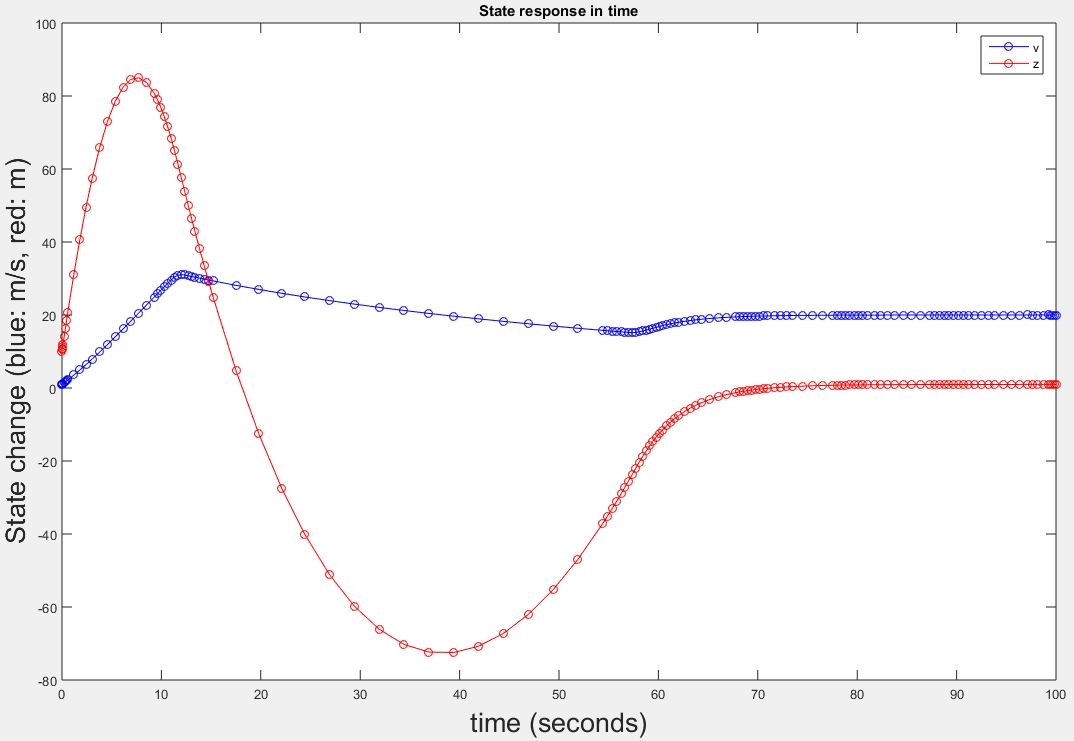
\includegraphics[width=0.8\textwidth]{A2_state_time.jpg}
\caption{States change in time}
\end{figure}
\end{center}

\clearpage

Below are several views of the corresponding phase portrait; with different levels of zoom to show the effect of the controller trying to reach a desired negative velocity (remember torque can only be positive, there is no reverse) which results in instability. In addition, there is a asymptotically stable equilibrium where V = Vr (= 20) and a corresponding integral state.


\begin{center}
\begin{figure}[htb]
	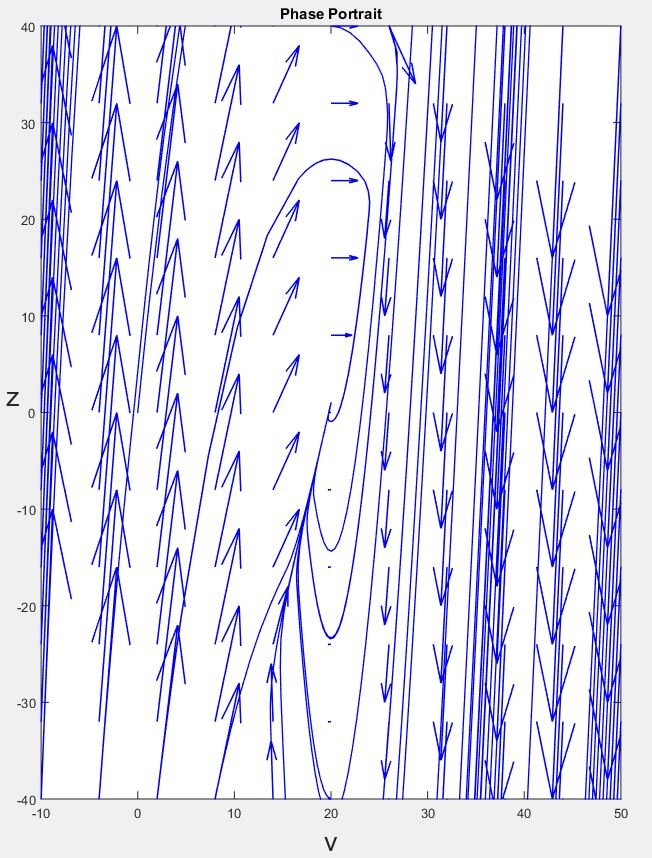
\includegraphics[width=0.6\textwidth]{A2_phaseportrait_1.jpg}
\caption{Phase Portrait of state variables v and z - note the stable equilibrium point at the regulated velocity}
\end{figure}
\end{center}


\clearpage

Zooming out further, it appears that the phase portrait represents a stable spiral for all initial conditions.


\begin{center}
\begin{figure}[htb]
	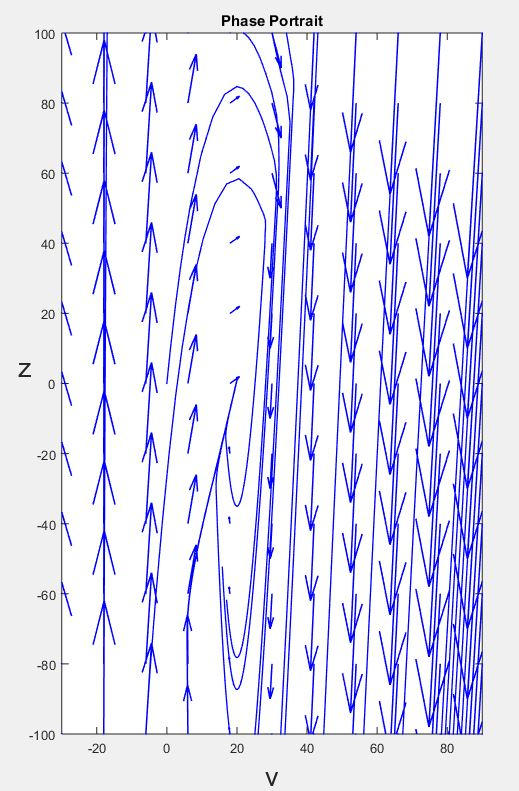
\includegraphics[width=0.6\textwidth]{A2_phaseportrait_2.jpg}
\caption{Phase Portrait of state variables v and z - note the stable equilibrium point at the regulated velocity}
\end{figure}
\end{center}

\clearpage

However, this is not true, it can be seen that for large velocities, where the angular velocity is exceeded for gear 3, it is indeterminable as to whether the trajectories return to the aforementioned equilibrium. This is shown in the figure below, which also shows that for negative velocities the system is unstable, as all initial conditions result in the two states growing with time.



\begin{center}
\begin{figure}[htb]
	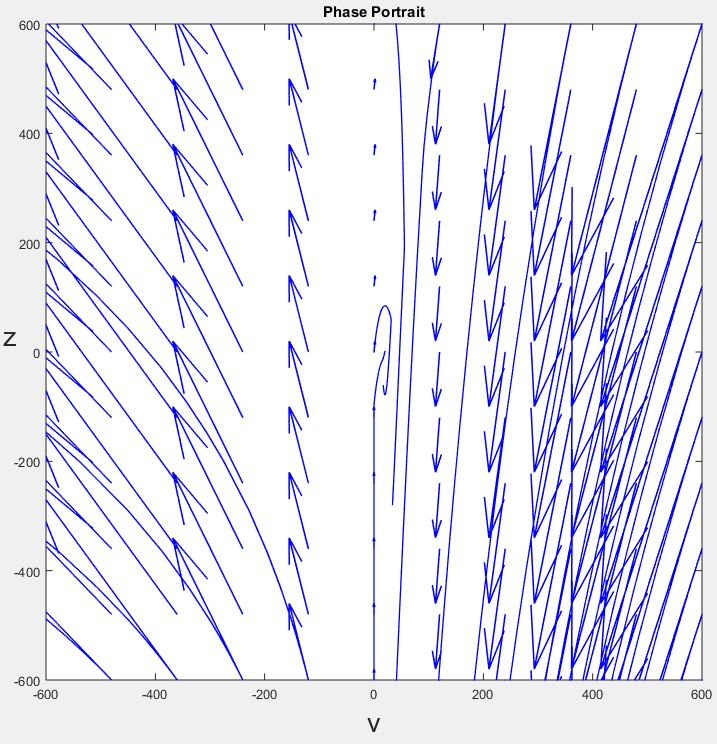
\includegraphics[width=0.6\textwidth]{A2_phaseportrait_3.jpg}
\caption{Phase Portrait of state variables v and z - illustrates the unstable and stable regions of the two states v and z}
\end{figure}
\end{center}


The position of the stable equilibrium is positioned at $v = 20$, as found when reviewing the figures above (in particular figure 1). The corresponding value of $z$ is harder to recognise, however from vooming into figure 1 for large time (90-100 seconds), it can be seen that $z$ is reaching a steady state value of approximately $z = 0.97$, as shown in the figure below, and recognisable in figure 2 as the point where all lines meet (and $v=20$).


\begin{center}
\begin{figure}[htb]
	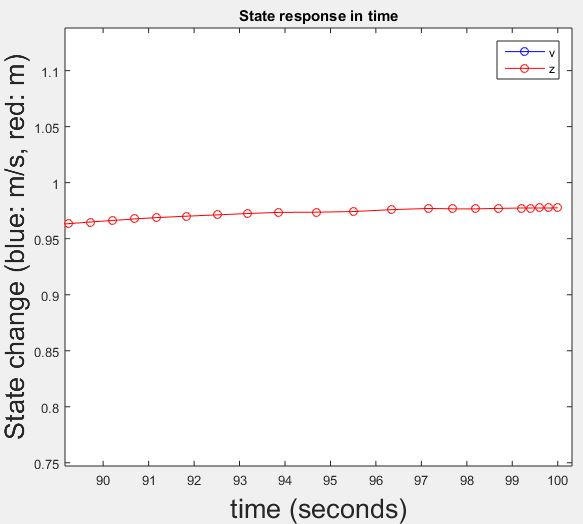
\includegraphics[width=0.6\textwidth]{A2_state_time_zoom.jpg}
\caption{Steady State Response of 'z'}
\end{figure}
\end{center}

\clearpage


\section{Question 2}

From the previous assignment, it is known that;

\vspace{\baselineskip}

$T(\omega, \lambda) = \lambda * T_m *(1-\beta *(\frac{\omega}{\omega_m} - 1)^2)$

\vspace{\baselineskip}

$\lambda = sat(u) $

\vspace{\baselineskip}

$u = K_p (v_r - v) + K_i \int_{0}^{t} (v_r - v) d \tau$

\vspace{\baselineskip}

$F_{applied} = \alpha T(\omega, \lambda)$

\vspace{\baselineskip}

$F_{total} = F_{applied} - (m g C_r sign(v) + \frac{1}{2} \rho C_d A v^2$

\vspace{\baselineskip}

$\therefore F_{total} = m*a = F_{applied} - F_{disturbance}$

\vspace{\baselineskip}

$\rightarrow v' = \frac{F_{applied}}{m} - g*C_r*sign(v) - \frac{1}{2*m} \rho C_d  A v^2$
 
\vspace{\baselineskip} 
 
where $F_d = g*C_r*sign(v) + \frac{1}{2*m} \rho C_d A*v^2 $
v' can be written as; 

\vspace{\baselineskip}

$v' = \frac{\alpha}{m} sat(K_p (v_r - v) + K_i z) T_m (1-\beta (frac{\omega}{\omega_m}- 1)^2) - Fd$

\vspace{\baselineskip}

as $z$ is the integral state of the controller, or the integral of the error between the regulated velocity and the actual velocity, $z'$ is the derivative of the integral of the error. Thus, $z$ is simply the error in velocity;

\vspace{\baselineskip}

$z = v_r - v$

\vspace{\baselineskip}

Thus, the state-space equation, $x' = F(x)$, can be formed;

\vspace{\baselineskip}

$\begin{bmatrix}
  v' \\
  z'  \\ 
  \end{bmatrix}
  = 
  \begin{bmatrix}
  \frac{\alpha}{m}  sat(K_p (v_r - v) + K_i z)  T_m (1-\beta (\frac{\omega}{\omega_m}- 1)^2) - (g C_r sign(v) + \frac{1}{2*m} \rho C_d A*v^2) \\
  v_r - v  \\ 
  \end{bmatrix}
$

\vspace{\baselineskip}

Systems have equilibrium points where the states stop changing in time; as seem in part 1 of this assignment, stable systems state's can reach a steady-state value. Thus, there exists values of $x = [v, z]$ such that $[v', z'] = [0, 0] = F(x)$.

Computing row two of the state-space equation for $v$ corresponding to $v' = 0$ gives;

\vspace{\baselineskip}

$0 = v_r - v$

$\therefore v = v_r$

\vspace{\baselineskip}

similarly, row one can be solved for $z$ give it is known that an equilibrium point is at $v = v_r$

\vspace{\baselineskip}

$ 0 = \frac{\alpha}{m} * u * T_m * (1-\beta (\frac{\omega}{\omega_m}- 1)^2) - F_d$

\vspace{\baselineskip}

$ 0 = \frac{\alpha}{m} * [K_p (v_r - v_r) + K_i z] * T_m * (1-\beta (\frac{\omega}{\omega_m}- 1)^2) - F_d$

\vspace{\baselineskip}

$\therefore z = \frac{m * F_d}{\alpha K_i T_m (1-\beta (\frac{\omega}{\omega_m}- 1)^2)} $

\vspace{\baselineskip}

thus, there is an equilibrium point at;

\vspace{\baselineskip}

$[v, z] = [ v_r, \frac{m * F_d}{\alpha K_i T_m (1-\beta (\frac{\omega}{\omega_m}- 1)^2)} ]$

\vspace{\baselineskip}

Checking that V(x) is a Lyapunov function for the non-linear system requires computation of a formula which only holds if the equilibrium is at the origin; $[v, z] = [0, 0]$. Additionally, the eigenvalues of A can be used to test if the origin is asymptotically stable; if they have negative and real parts. Thus, to determine whether the system is stable by Lyapunov, a change in coordinates is required.

For this, $x$ and $y$ will define the new coordinate system such that;

\vspace{\baselineskip}

$x = v - v_r$ and $y = z - \frac{m * F_d}{\alpha K_i T_m (1-\beta (\frac{\omega}{\omega_m}- 1)^2)} $

\vspace{\baselineskip}

Thus, $F(x)$ is now a function of $[x, y]$, and the state-space input equation can be rewritten.

Matlab is used for the following computations, as they become quite complicated. The final code is illustrated in the figure below, sections are seperated by $%%$, and a detailed walk through of it follows;

\vspace{\baselineskip}


\lstinputlisting[caption={PBA2\_2\_3script.m}]{PBA2_2_3script.m}

\vspace{\baselineskip}

In the third line of code, all of the cruise control variables are defined as real and  symbolic; so they can be carried through equations.

The equation for $\lambda$ is then defined, assuming small $u$, such that there is no saturation required. Following, the equation for torque and disturbance forces are represented by $T$ and $Fd$ respectively.

The state-space equation is then written for $[v', z'] = F([v, z])$, as calculated above. From this, the change of coordinate system is performed to calculate $[x', y'] = F([x, y])$, denoted $F\_xy$, and the $x$ and $y$ terms are collected such that $F\_xy$ is written with the variable order factored. This results in;

\vspace{\baselineskip}

$x' = $
$
\begin{array}{c} \frac{\left(\mathrm{Kp}\, \mathrm{Tm}\, {\mathrm{alpha}}^3\, \mathrm{beta}\right)}{\left(m\, {\mathrm{wm}}^2\right)}\, x^3 + -\frac{\mathrm{Ki}\, \mathrm{Tm}\, {\mathrm{alpha}}^3\, \mathrm{beta}}{m\, {\mathrm{wm}}^2}\, x^2\, y + -\frac{\mathrm{Kp}\, \mathrm{Tm}\, \mathrm{alpha}\, \left(2\, \mathrm{alpha}\, \mathrm{beta}\, \mathrm{wm} - 2\, \mathrm{Vr}\, {\mathrm{alpha}}^2\, \mathrm{beta}\right)}{m\, {\mathrm{wm}}^2}\, x^2 
\end{array}$

$ \begin{array}{c}
+ \frac{\left(\mathrm{Ki}\, \mathrm{Tm}\, \mathrm{alpha}\, \left(2\, \mathrm{alpha}\, \mathrm{beta}\, \mathrm{wm} - 2\, \mathrm{Vr}\, {\mathrm{alpha}}^2\, \mathrm{beta}\right)\right)}{\left(m\, {\mathrm{wm}}^2\right)}\, x\, y + 
\end{array}$

$\begin{array}{c}
\frac{\left(\mathrm{Kp}\, \mathrm{Tm}\, \mathrm{alpha}\, \left(\mathrm{beta}\, {\mathrm{wm}}^2 - {\mathrm{wm}}^2 + {\mathrm{Vr}}^2\, {\mathrm{alpha}}^2\, \mathrm{beta} - 2\, \mathrm{Vr}\, \mathrm{alpha}\, \mathrm{beta}\, \mathrm{wm}\right)\right)}{\left(m\, {\mathrm{wm}}^2\right)}\, x +
\end{array}$

$\begin{array}{c}
 -\frac{\mathrm{Ki}\, \mathrm{Tm}\, \mathrm{alpha}\, \left(\mathrm{beta}\, {\mathrm{wm}}^2 - {\mathrm{wm}}^2 + {\mathrm{Vr}}^2\, {\mathrm{alpha}}^2\, \mathrm{beta} - 2\, \mathrm{Vr}\, \mathrm{alpha}\, \mathrm{beta}\, \mathrm{wm}\right)}{m\, {\mathrm{wm}}^2}\, y\\  \end{array}
$
                                                                                                                                                                                                                                                                                                                                                                                                           
                                                                                                                                                                                                                                                                                                                                                                                                           
                                                                                                                                                                                                                                                                                                                                                                                                            $ y' = -x $


\vspace{\baselineskip}

All represented by $F\_xy$, where the higher order terms are copied into a matrix $F\_$ in the following section, and the linear terms are stored in the matrix $A\_1$.

It can be seen from the above expressions that matrix $A\_1$ will contain a positive first row first column element (because of the sign infront of the x term), and a negative first row second column element (because of the sign in front of the y term). Computing A\_1 shows that the second row is $[ -1, 0 ]$, corresponding to the second equation above. 

Following this, a symbolic representation of the Lyuponuv function is computed, using the symbols $a\_11$ to denote the first (row and column) expression in $A\_1$, $a\_12$ denotes the expression in the first row and second column of $A\_1$. $As$, the symbolically simplified representation of $A\_$ is then formed; as seen in the Matlab code. 

From this, the $P$ matrix in the Lyapunov function can be defined and values computed using the Lyapunov equation;

\vspace{\baselineskip}

$ V(x) = x^T P x$

\vspace{\baselineskip}

$A^T P + P A = -Q$, 

\vspace{\baselineskip}

where $Q = I$; I is the identity matrix and Q is thus positive definite.

This is done in Matlab using the function $solve()$, which equates the above expression to find the coefficients of $P\_$; $P\_11$, $P\_12$ and $P\_22$. These are then reassigned into the P matrix, where the determinant, eigenvalues and trace of P are computed.

\vspace{\baselineskip}

$ P\_ = 
\left(\begin{array}{cc} -\frac{a_{12} - 1}{2\, a_{11}\, a_{12}} & \frac{1}{2\, a_{12}}\\ \frac{1}{2\, a_{12}} & \frac{{a_{11}}^2 + {a_{12}}^2 - a_{12}}{2\, a_{11}\, a_{12}} \end{array}\right)
$

\vspace{\baselineskip}

$EA\_=
\left(\begin{array}{c} \frac{a_{11}}{2} - \frac{\sqrt{{a_{11}}^2 + 4\, a_{12}}}{2}\\ \frac{a_{11}}{2} + \frac{\sqrt{{a_{11}}^2 + 4\, a_{12}}}{2} \end{array}\right)
$

\vspace{\baselineskip}

note that for the linear system to be asymptotically stable, A must have real, negative parts. From above, it can be seen that this is only possible if $a\_11$ is negative. (Which implies that the expression for $As$ would be better having $+ a\_11$ in the first element)

\vspace{\baselineskip}

$ D\_ =
-\frac{{a_{11}}^2 + {a_{12}}^2 - 2\, a_{12} + 1}{4\, {a_{11}}^2\, a_{12}}
$

\vspace{\baselineskip}

$E\_ =
\left(\begin{array}{c} \frac{{a_{11}}^2 - \sqrt{\left({a_{11}}^2 + {a_{12}}^2 - 2\, a_{11} + 1\right)\, \left({a_{11}}^2 + {a_{12}}^2 + 2\, a_{12} + 1\right)} - 2\, a_{12} + {a_{12}}^2 + 1}{4\, a_{11}\, a_{12}}\\ \frac{\sqrt{\left({a_{11}}^2 + {a_{12}}^2 - 2\, a_{12} + 1\right)\, \left({a_{11}}^2 + {a_{12}}^2 + 2\, a_{12} + 1\right)} - 2\, a_{12} + {a_{11}}^2 + {a_{12}}^2 + 1}{4\, a_{11}\, a_{12}} \end{array}\right)
$
  
\vspace{\baselineskip}  
  
$T\_ = 
\frac{{a_{11}}^2 + {a_{12}}^2 - 2\, a_{12} + 1}{2\, a_{11}\, a_{12}}
$

\vspace{\baselineskip}

It can be seen that the trace and determinant of $P$ are both negative given $a\_11 < 0$; however this can be fixed if both $a\_11$, $a\_12 < 0$. Additionally, this would give positive eigenvalues for P (expression $E\_$); implying the Lyapunov function is positive definite. This can be explained when analysing the $A\_1$ elements in detail, where it appears the negative terms in the expressions will be computed to be larger, thus making then negative and real, unlike that assumed. Nonetheless, the math will come out the same in the end.

Thus, assuming all coefficients are real and positive, potentially, a better A matrix to assume (for stability) could be;

\vspace{\baselineskip}

$A = \begin{bmatrix}
  -a_{11} & a_{12} \\
  -1      &   0	  \\ 
  \end{bmatrix}
$

\vspace{\baselineskip}

Following from this, the next section computes $P$ with the same method, but where the A matrix (denoted $A\_1$) contains the cruise control model parameters. The eigenvalues of P are then found by substituting in the model parameters used in part 1, giving positive real results of 0.3506 and 3.9294, with a trace of 4.28. Similarly, it was seen that A contained negative eigenvalues, implying the linearised model is asymptotically stable.

To check if the proposed Lyapunov function is valid for the non-linear system, the following function need be computed using the matrix comprising of the higher order terms of F([x, y]);

\vspace{\baselineskip}

$\lim_{||x|| \rightarrow 0} \frac{||F(x)||}{||x||} = 0$

\vspace{\baselineskip}

This is computed in the next section of code in two ways, using the limit function, and calculating the limit manually where $[x, y] = [0.00000001, 0.00000001]$. Both of these arrive at the same result, that the limit goes to 0; however the latter test shows that the numerator goes to 0 first, and thus the solution is determinant, as proved by the limit function.

The Lyapunov function for the used P in the code, with all model parameters, and with the substitution, are displayed further down in the code image.
Where the symbolic $V(x)$ came to be;

\vspace{\baselineskip}

$ V(x) =
\left(\frac{1 - a_{12}}{2\, a_{11}\, a_{12}}\right)\, x^2 + \frac{x\, y}{a_{12}} + \left(\frac{{a_{11}}^2 + {a_{12}}^2 - a_{12}}{\left(a_{11}\, a_{12}\, *2\right)}\right)\, y^2
$

\vspace{\baselineskip}

which assuming both $a\_11$ and $a\_12$ are negative, as determined earlier, produces a positive Lyapunov function for the cruise control system; if $[x, y] > 0$.

The symbolic and parameter solutions were equated in the end of the Matlab code, that verified that they were equal.



\clearpage

\end{document}